% Options for packages loaded elsewhere
\PassOptionsToPackage{unicode}{hyperref}
\PassOptionsToPackage{hyphens}{url}
\PassOptionsToPackage{dvipsnames,svgnames,x11names}{xcolor}
%
\documentclass[
  letterpaper,
  DIV=11,
  numbers=noendperiod]{scrartcl}

\usepackage{amsmath,amssymb}
\usepackage{lmodern}
\usepackage{iftex}
\ifPDFTeX
  \usepackage[T1]{fontenc}
  \usepackage[utf8]{inputenc}
  \usepackage{textcomp} % provide euro and other symbols
\else % if luatex or xetex
  \usepackage{unicode-math}
  \defaultfontfeatures{Scale=MatchLowercase}
  \defaultfontfeatures[\rmfamily]{Ligatures=TeX,Scale=1}
\fi
% Use upquote if available, for straight quotes in verbatim environments
\IfFileExists{upquote.sty}{\usepackage{upquote}}{}
\IfFileExists{microtype.sty}{% use microtype if available
  \usepackage[]{microtype}
  \UseMicrotypeSet[protrusion]{basicmath} % disable protrusion for tt fonts
}{}
\makeatletter
\@ifundefined{KOMAClassName}{% if non-KOMA class
  \IfFileExists{parskip.sty}{%
    \usepackage{parskip}
  }{% else
    \setlength{\parindent}{0pt}
    \setlength{\parskip}{6pt plus 2pt minus 1pt}}
}{% if KOMA class
  \KOMAoptions{parskip=half}}
\makeatother
\usepackage{xcolor}
\setlength{\emergencystretch}{3em} % prevent overfull lines
\setcounter{secnumdepth}{-\maxdimen} % remove section numbering
% Make \paragraph and \subparagraph free-standing
\ifx\paragraph\undefined\else
  \let\oldparagraph\paragraph
  \renewcommand{\paragraph}[1]{\oldparagraph{#1}\mbox{}}
\fi
\ifx\subparagraph\undefined\else
  \let\oldsubparagraph\subparagraph
  \renewcommand{\subparagraph}[1]{\oldsubparagraph{#1}\mbox{}}
\fi


\providecommand{\tightlist}{%
  \setlength{\itemsep}{0pt}\setlength{\parskip}{0pt}}\usepackage{longtable,booktabs,array}
\usepackage{calc} % for calculating minipage widths
% Correct order of tables after \paragraph or \subparagraph
\usepackage{etoolbox}
\makeatletter
\patchcmd\longtable{\par}{\if@noskipsec\mbox{}\fi\par}{}{}
\makeatother
% Allow footnotes in longtable head/foot
\IfFileExists{footnotehyper.sty}{\usepackage{footnotehyper}}{\usepackage{footnote}}
\makesavenoteenv{longtable}
\usepackage{graphicx}
\makeatletter
\def\maxwidth{\ifdim\Gin@nat@width>\linewidth\linewidth\else\Gin@nat@width\fi}
\def\maxheight{\ifdim\Gin@nat@height>\textheight\textheight\else\Gin@nat@height\fi}
\makeatother
% Scale images if necessary, so that they will not overflow the page
% margins by default, and it is still possible to overwrite the defaults
% using explicit options in \includegraphics[width, height, ...]{}
\setkeys{Gin}{width=\maxwidth,height=\maxheight,keepaspectratio}
% Set default figure placement to htbp
\makeatletter
\def\fps@figure{htbp}
\makeatother

\usepackage{booktabs}
\usepackage{longtable}
\usepackage{array}
\usepackage{multirow}
\usepackage{wrapfig}
\usepackage{float}
\usepackage{colortbl}
\usepackage{pdflscape}
\usepackage{tabu}
\usepackage{threeparttable}
\usepackage{threeparttablex}
\usepackage[normalem]{ulem}
\usepackage{makecell}
\usepackage{xcolor}
\KOMAoption{captions}{tableheading}
\makeatletter
\makeatother
\makeatletter
\makeatother
\makeatletter
\@ifpackageloaded{caption}{}{\usepackage{caption}}
\AtBeginDocument{%
\ifdefined\contentsname
  \renewcommand*\contentsname{Table of contents}
\else
  \newcommand\contentsname{Table of contents}
\fi
\ifdefined\listfigurename
  \renewcommand*\listfigurename{List of Figures}
\else
  \newcommand\listfigurename{List of Figures}
\fi
\ifdefined\listtablename
  \renewcommand*\listtablename{List of Tables}
\else
  \newcommand\listtablename{List of Tables}
\fi
\ifdefined\figurename
  \renewcommand*\figurename{Figure}
\else
  \newcommand\figurename{Figure}
\fi
\ifdefined\tablename
  \renewcommand*\tablename{Table}
\else
  \newcommand\tablename{Table}
\fi
}
\@ifpackageloaded{float}{}{\usepackage{float}}
\floatstyle{ruled}
\@ifundefined{c@chapter}{\newfloat{codelisting}{h}{lop}}{\newfloat{codelisting}{h}{lop}[chapter]}
\floatname{codelisting}{Listing}
\newcommand*\listoflistings{\listof{codelisting}{List of Listings}}
\makeatother
\makeatletter
\@ifpackageloaded{caption}{}{\usepackage{caption}}
\@ifpackageloaded{subcaption}{}{\usepackage{subcaption}}
\makeatother
\makeatletter
\@ifpackageloaded{tcolorbox}{}{\usepackage[many]{tcolorbox}}
\makeatother
\makeatletter
\@ifundefined{shadecolor}{\definecolor{shadecolor}{rgb}{.97, .97, .97}}
\makeatother
\makeatletter
\makeatother
\ifLuaTeX
  \usepackage{selnolig}  % disable illegal ligatures
\fi
\IfFileExists{bookmark.sty}{\usepackage{bookmark}}{\usepackage{hyperref}}
\IfFileExists{xurl.sty}{\usepackage{xurl}}{} % add URL line breaks if available
\urlstyle{same} % disable monospaced font for URLs
\hypersetup{
  pdftitle={STAT 210 Parsons' Paper Company Workers Database},
  pdfauthor={Lorraine Oloo and Camden Heafitz},
  colorlinks=true,
  linkcolor={blue},
  filecolor={Maroon},
  citecolor={Blue},
  urlcolor={Blue},
  pdfcreator={LaTeX via pandoc}}

\title{STAT 210 Parsons' Paper Company Workers Database}
\author{Lorraine Oloo and Camden Heafitz}
\date{2023-03-03}

\begin{document}
\maketitle
\ifdefined\Shaded\renewenvironment{Shaded}{\begin{tcolorbox}[sharp corners, frame hidden, breakable, interior hidden, enhanced, borderline west={3pt}{0pt}{shadecolor}, boxrule=0pt]}{\end{tcolorbox}}\fi

\renewcommand*\contentsname{Table of contents}
{
\hypersetup{linkcolor=}
\setcounter{tocdepth}{3}
\tableofcontents
}
\hypertarget{introduction}{%
\subsection{Introduction}\label{introduction}}

Mining the History of Holyoke (STAT210) is a class at Amherst College
with a mission statement of curating and publishing a piece of Holyoke's
history and making it accessible to the town's people. One way our class
has begun this journey is by analyzing and curating an old payroll
registry found in an attic in Holyoke and now available in the archives
of the Holyoke Public Library History Room. This register tracked pay
for employees who worked at the Parsons Paper Mill in Holyoke,
Massachusetts (the ``Paper City'') in the 1860s.

It has been remarkable to track down so much history as each page of
this nearly 400 page registry has upwards of 30 employees, and each name
has its own story worth telling. In the registry, we can see the name,
number of days worked, their wages, whether or not the worker had rent
or board due, the final balance owed, and signature (see
Figure~\ref{fig-sample1}). Click
\href{https://r.amherst.edu/apps/nhorton/Parsons-Paper/}{here} for an
interactive display of the register.

\hypertarget{workers-summary}{%
\subsection{Workers' Summary}\label{workers-summary}}

We took on the task of finding more information about some of the
employees at the paper mill using the gyneological database
Ancestry.com. On page 259, we found two women with the same last name
(see Figure~\ref{fig-sample2}) which was common back then and decided to
search for them on Ancestry.com. Their names were Lucy and E.A. Allen.

When we searched for Lucy, we found that E.A. stood for Eliza Ann
Allen--they were sisters! (see Figure~\ref{fig-sample2}). Lucy was born
in Massachusetts in 1842 and Eliza Ann was her older sister born in
1841. They lived in dwelling 42. Their father's name was Job Allen and
their mother was Anna Allen. Job was born in England and moved to the
United States sometime before 1841. Like his daughters, he too worked at
the Parsons Paper Company. We found record of him first on page 3. (see
Figure~\ref{fig-sample3}). Anna Allen stayed at home. This was a common
life for a working-class family in Holyoke, Massachusetts in the 1860s.

From what we were able to gather, Eliza and Lucy were finishers meaning
they helped with finalizing the paper making process. We made this
assumption when we found Lucy's name on Page 2 under the label
``Finishers.'' See (Figure~\ref{fig-sample4}). Eliza and Lucy were paid
not by the number of hours or days they worked but rather the number of
reams they finished. We can see on page on page 2 that Lucy finished 756
reams of paper for the month of January in 1861. Eliza's name first
appeared in 1862 on page 34 right below her sisters name, one year after
her sister first started working. (see Figure~\ref{fig-sample5}).
Coincidentally, they were one year apart in age. Perhaps their father
Job did not want his daughters to work until they were 20 years of age.

It seemed that the Allen family had trouble finding a permanent
residence as we found a number of addresses reported across different
resources. In 1869, the Holyoke city directory shows that the Allen
family lived on Dwight Street. Ancestry.com showed that the Allen family
lived in dwelling 42 with no street name reported in 1870. (see
Figure~\ref{fig-sample6}). We were able to follow Lucy's places of
residence in several years after 1870 until her death on May 11, 1893 in
Holyoke, MA. See Figure~\ref{fig-sample7} for Lucy's places of
residence.

Following the inspection of the payroll pages (pg 1-319) of the PPP
register, we observe that Lucy, Eliza, and Job all worked throughout the
decade. It is reasonable to presume that the Allen daughter were
unlikely to be pursing education on this time. Lucy also appears to have
continued working in the PPC mill until her death. It is difficult to
determine if the Allen family's literacy due to inconsistencies in
signatures. Some signatures have ``X'' in them while others do not, and
the handwriting is different across the decade suggesting they multiple
people could have been signing for them.

Additionally, we were able to find records on Joseph Clark Parsons; the
founder of the Parsons Paper Company (see Figure~\ref{fig-sample8}). We
chose to explore his ancestry and observe how it would differ to those
of his employees.

Parsons was born on February 6, 1814, in Northampton, Hampshire County,
Massachusetts to Lydia and Justice Parsons. Parsons was a local
businessman who became very successful after founding his mill. He
married Lucretia Hoyt Parsons and had three daughters; Catherine Turner
Taft, Fannie Colton Parsons, and Elizabeth Hoyt Parsons. We found that
Parsons lived in house 22 of dwelling 165 on Suffolk street which was
quite close to his Mill. This was surprising because we expected him to
live in the upper-class district because wealthier people lived in hills
above sea level.

If we continued our research, we would aim to find descendants of the
Parsons Paper Company that are still living today.

\hypertarget{photo-references}{%
\subsection{Photo References}\label{photo-references}}

\begin{figure}

{\centering \includegraphics[width=9.8in,height=0.47\textheight]{Registry_page_header.jpeg}

}

\caption{\label{fig-sample1}This is page 259 of the PPP registry,
demonstrating how the name, days worked, wages, whether or not the
worker had rent or board due, final balance owed, and signature were
recorded}

\end{figure}

\begin{figure}

{\centering \includegraphics[width=0.7\textwidth,height=\textheight]{Mary and Eliza Allen.jpeg}

}

\caption{\label{fig-sample2}Lucy and Eliza Ann Allen entries in the
Registry page 259. March 1st, 1868}

\end{figure}

\begin{figure}

{\centering \includegraphics[width=0.7\textwidth,height=\textheight]{Job Allen page 3 .png}

}

\caption{\label{fig-sample3}Job Allen in the Registry page 3, line 5.
February 1st, 1861. In this pay period he worked 27 days and received
\$31}

\end{figure}

\begin{figure}

{\centering 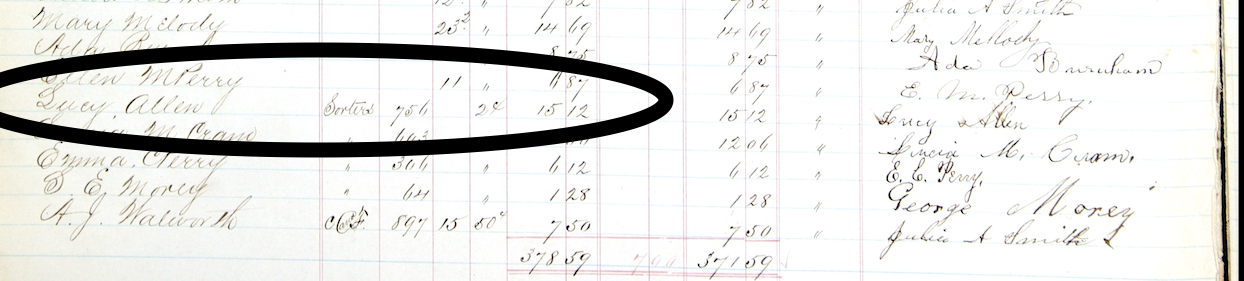
\includegraphics[width=0.9\textwidth,height=\textheight]{Lucypg2.png}

}

\caption{\label{fig-sample4}Lucy Allen in the Registry page 2, line 3.
January, 1861. In this pay period she worked 24 and received \$15.12}

\end{figure}

\begin{figure}

{\centering \includegraphics[width=0.9\textwidth,height=\textheight]{Eliza and lucy allen page 34.png}

}

\caption{\label{fig-sample5}Lucy and Eliza Ann Allen on page 34 line 5
and 6. January, 1862}

\end{figure}

\begin{figure}

{\centering \includegraphics[width=0.5\textwidth,height=\textheight]{Lucy_Allen.jpeg}

}

\caption{\label{fig-sample6}Lucy Allen's Profile from Ancestry.com
providing details on her birth year and family members}

\end{figure}

\begin{figure}

{\centering \includegraphics[width=9.36in,height=0.4\textheight]{Joseph_Clark.jpeg}

}

\caption{\label{fig-sample8}Joseph C. Parsons' Profile (1814-1886)}

\end{figure}

\clearpage

\begin{figure}

{\centering 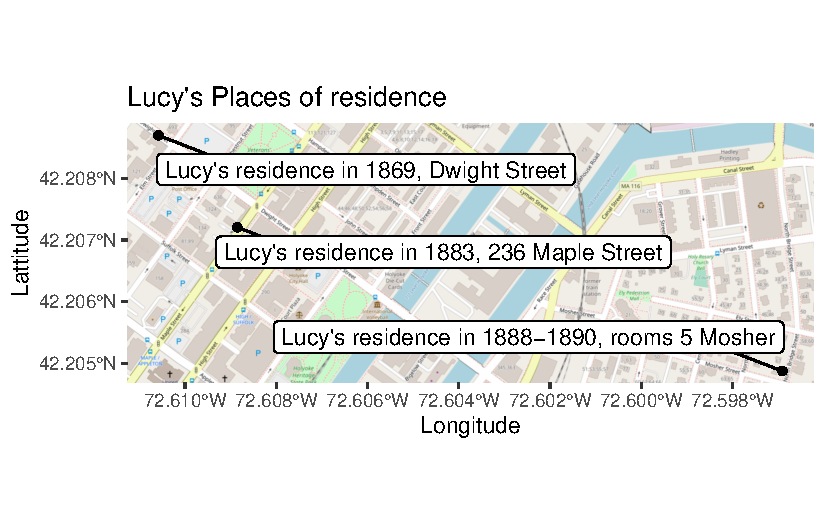
\includegraphics{workers_database_files/figure-pdf/fig-sample7-1.pdf}

}

\caption{\label{fig-sample7}The black dots shows the 3 residences for
Lucy Allen from years 1869-90}

\end{figure}

\hypertarget{database}{%
\subsection{Database}\label{database}}

Here\ref{table} is the database we created. It displays personal
information about Parson's Paper employees. We can find who they are,
when they were born, their address, family members, and place of origin.
Naturally, with data this old, we could not find each and every piece of
information for all of the employees. This is just a start that will
hopefully fuel other individuals to contribute to this document. If we
had extended time and resources, we would search up more employees on
Ancestry.com and try and find their living descendants today. For this
project, we were only able to access basic information on Ancestry.com.
It would be great to access the full database and find more
documentation of the employees as each additional document provides more
information about someone's life that we might not have had before. The
table shown below shows some of the columns of the data set. More
information is viewable in the full spreadsheet. This is the aggregated
info for some of the workers who worked in Parsons' paper in the 1860s:

\begin{table}

\caption{\label{table}Aggregated Data from Employees on Page 253 of the Registry From Ancestry.com}
\centering
\resizebox{\linewidth}{!}{
\begin{tabular}[t]{l|l|l|l|l}
\hline
Last Name & Birthday & Death Day & Spouse & Birthplace\\
\hline
Strick & 1859 & N/A & N/A & Chicopee, Mass\\
\hline
Parsons & 2/6/1814 & 3/12/1886 & Lucretia Hoyt Parsons & Northampton, Hampshire County, Massachusetts\\
\hline
Kelly & 1834 & N/A & Catherine Kelly & Ireland\\
\hline
Casey & 1843 & N/A & Ann Casey & Ireland\\
\hline
Kelley & 1840 & N/A & Hanna Kelley & Ireland\\
\hline
Hollom & 1835 & N/A & Ann Hollom & Ireland\\
\hline
Corner & 1849 & N/A & Anna Corner & Ireland\\
\hline
Mitchell & 1852 & N/A & N/A & MA\\
\hline
Allen & 1842 & N/A & N/A & MA\\
\hline
Allen & 1841 & N/A & N/A & MA\\
\hline
Allen & 1806 & N/A & Anna Ellen & England\\
\hline
William & 1849 & 12/12/1912 & Magaret Kelly & Ireland\\
\hline
Martin & 2/7/1838 & 11/11/1907 & Barbara F. Kelly & Crusheen, County Clare, Ireland\\
\hline
James & 4/4/1852 & 8/12/1915 & Mary O'Brien & Monson, Hampden, Massachusetts, USA\\
\hline
Thos & 1856 & N/A & N/A & N/A\\
\hline
Phillip & 1843 & 10/22/1902 & Ann Gilday & Ireland\\
\hline
John & 1843 & 2/23/1907 & Octavia Bordeaux Beaudry & Canada\\
\hline
Frank & N/A & 1853 & Lillian Short & Massachusetts\\
\hline
John & 1836 & 11/27/1922 & Mary Kelliher & Ireland\\
\hline
William & 1843 & 1930 & Florence Nightingale Growden & Maryhill, Lanarkshire, Scotland\\
\hline
Chester & 1819 & 4/18/1892 & Sarah Cooley & Easthampton, Hampshire, Massachusetts, USA\\
\hline
Martin & 6/24/1827 & 9/2/1903 & Emily Louisa Moore & Petersham, Worcester County, Massachusetts, United States\\
\hline
\end{tabular}}
\end{table}

\clearpage

\hypertarget{technical-appendix}{%
\subsection{\texorpdfstring{\textbf{Technical
Appendix}}{Technical Appendix}}\label{technical-appendix}}

The goal of this technical appendix is to provide a repeatable procedure
of our process of collecting the information from Ancestry.com so that
other passionate historians can build off our work. First, we accessed
the Amherst College Library account for Ancestry.com.

\begin{figure}

{\centering \includegraphics[width=9.51in,height=0.3\textheight]{amherst_website.png}

}

\caption{\label{fig-sample9}Once on the Amherst website, we clicked the
link to Ancestry Library Edition}

\end{figure}

The link to Amherst's access to ancestry website is
\href{https://libguides.amherst.edu/c.php?g=944984\&p=6812570}{here}.

Here is how the ancestry website looks at a first glance:

\begin{figure}

{\centering \includegraphics[width=9.6in,height=0.325\textheight]{website.jpeg}

}

\caption{\label{fig-sample10}Ancestry.com `search' screen}

\end{figure}

By searching for a name and a place, (Holyoke, Hampden, Massachusetts),
we were able to find census information from the 1800s and track down
paper mill workers.

The are a number of names that appear in first search. We used educated
guesses to select the most appropriate person looking at dates of birth
and death, places lived, and any other information that might've given
us a clue.

\begin{figure}

{\centering \includegraphics[width=9.31in,height=0.33\textheight]{multiple_names.jpeg}

}

\caption{\label{fig-sample11}Initial search results}

\end{figure}

The amount of information we could find on each worker varied from name
to name but in general, we were able to find birth year, birthplace,
spouse, children, parents, occupation, and address. Here is what Eliza
Ann's profile looks like on Ancestry.com. We then compiled these results
into this table\ref{table}.

\begin{figure}

{\centering \includegraphics[width=0.5\textwidth,height=\textheight]{ELIZA_ANN.png}

}

\caption{\label{fig-sample12}Eliza Ann Allen's Profile (1841-?)}

\end{figure}

\begin{figure}

{\centering 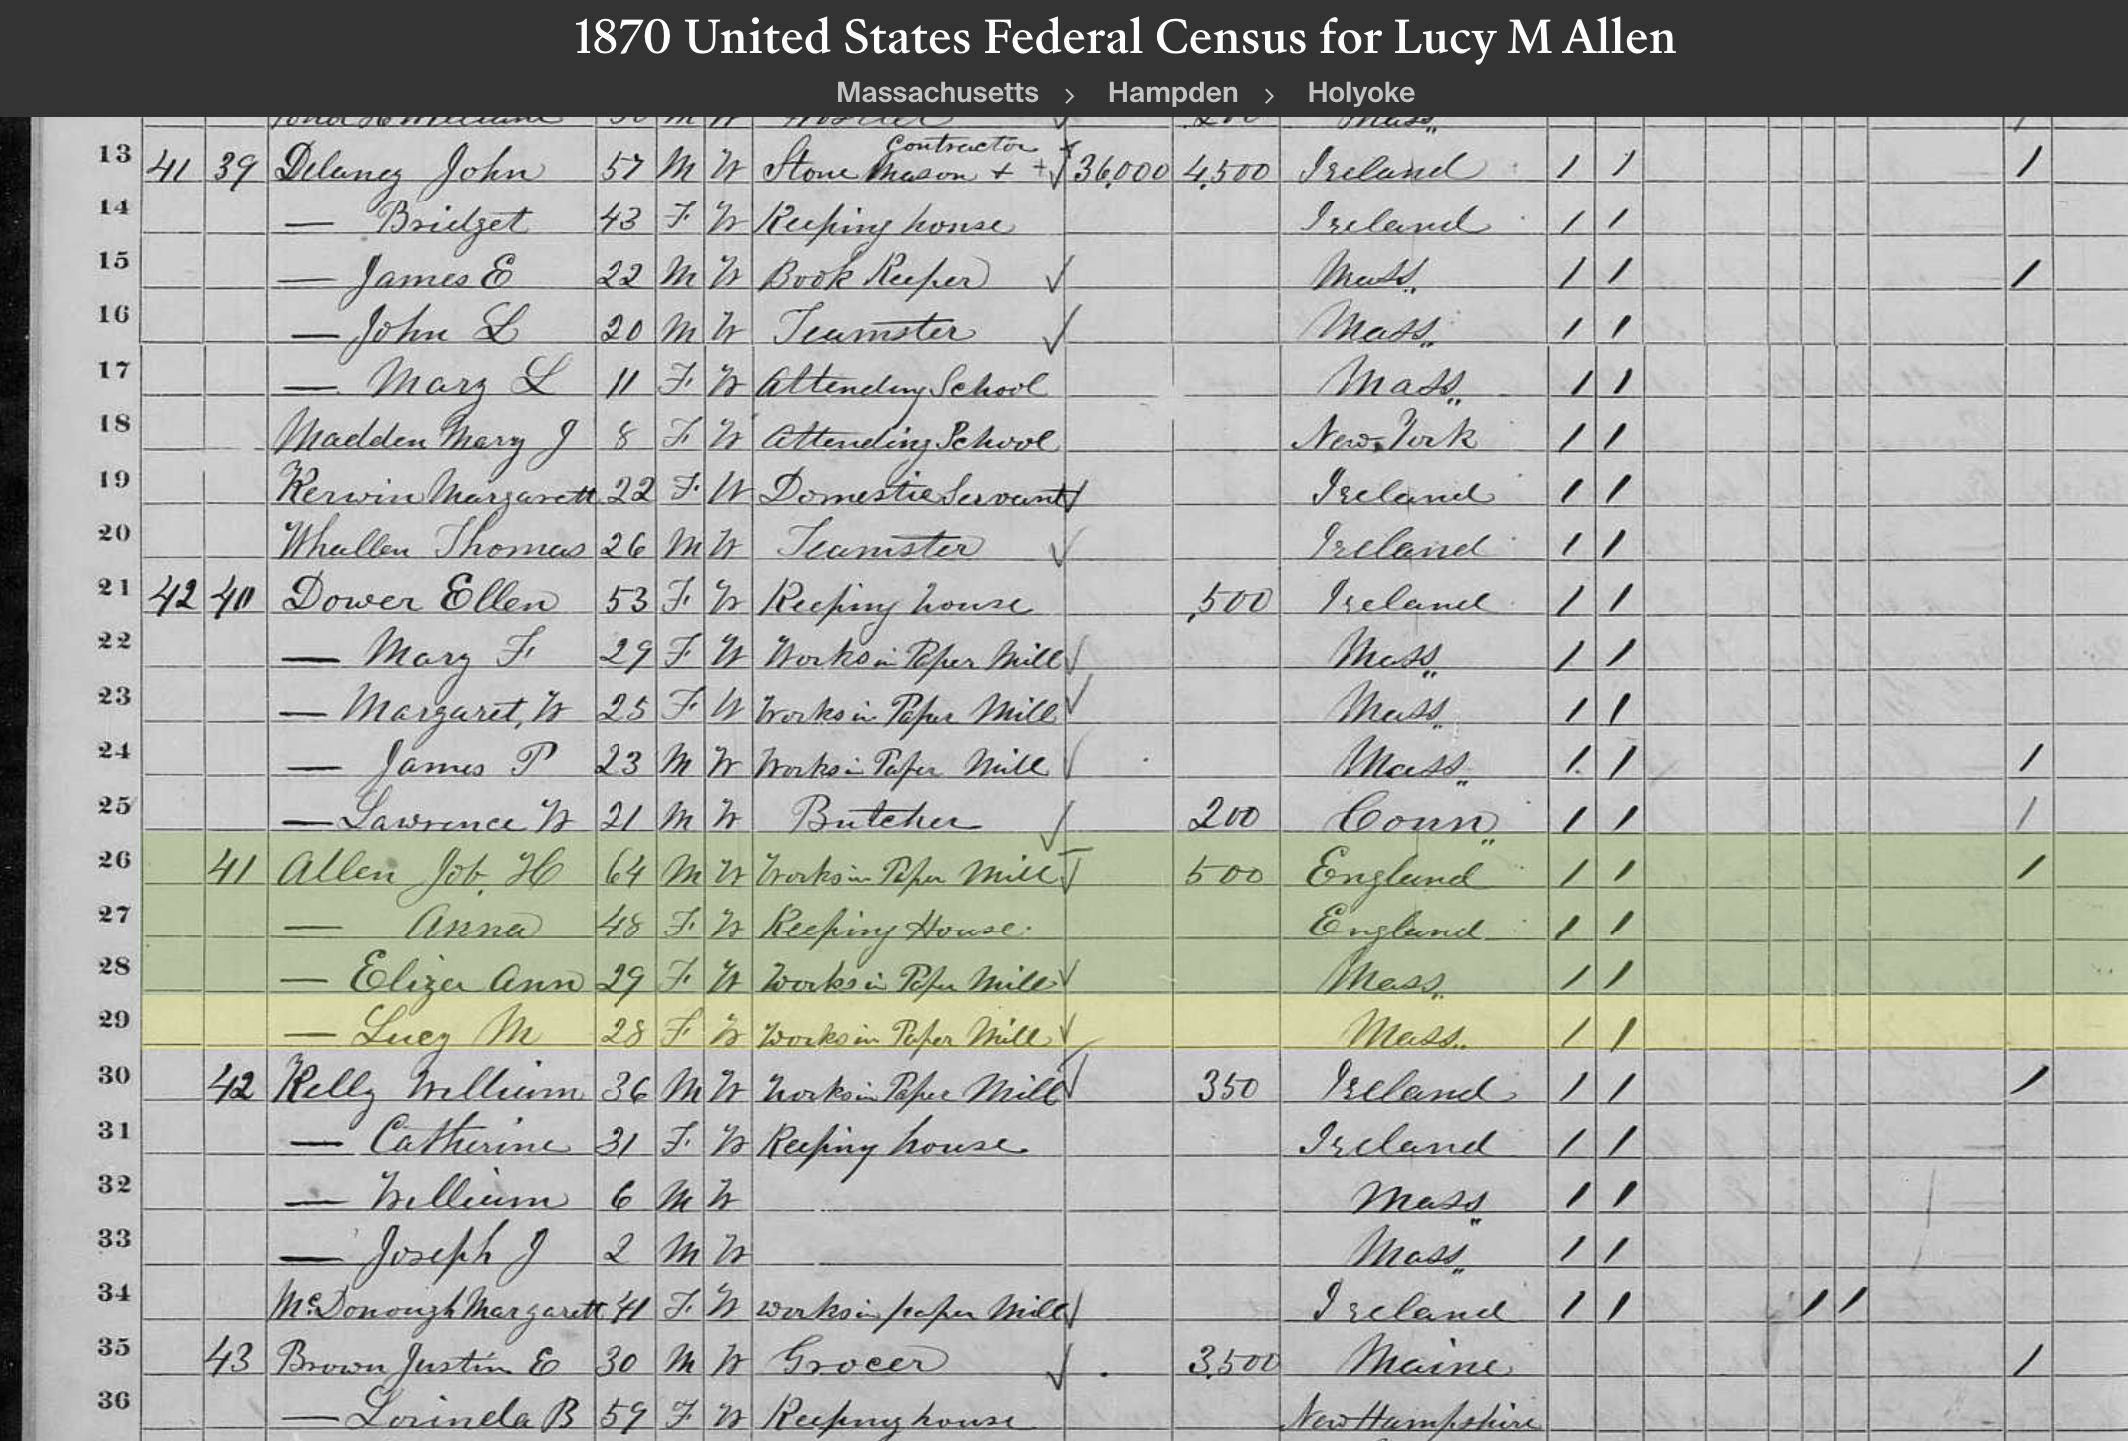
\includegraphics[width=0.7\textwidth,height=\textheight]{Allens family 1870 census Data.png}

}

\caption{\label{fig-sample13}Zoomed in Image of the 1870 Census}

\end{figure}



\end{document}
